\title{Автоматизация транспортного предприятия}
\author{Бушкин А. (САПР-1.1н), \\
  Голубев А. (САПР-1.1п), \\
  Чечеткин И. (САПР-1.1п)}
\institute{}
\date{}

\begin{frame}
  \titlepage
\end{frame}

\begin{frame}
%  \small
  Автоматизировать транспортное предприятие, осуществляющее перевозку грузов
  и пассажиров автомобильным транспортом по России. \textbf{Целью}
  автоматизации является снижение стоимости перевозок.
  
  \vspace{5mm}
  \textbf{Задачи:}
    \begin{itemize}
      \item исследование объекта;
      \item выделить слабые стороны рабочего процесса;
      \item выбрать самое подходящее решение проблемы.
    \end{itemize}
\end{frame}

\begin{frame}
  \frametitle{AS IS}
    \begin{figure}
      \center
      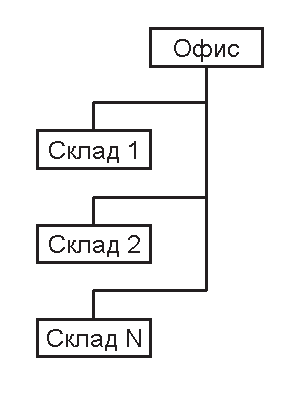
\includegraphics[width=.2\textwidth]{as_is_1}
      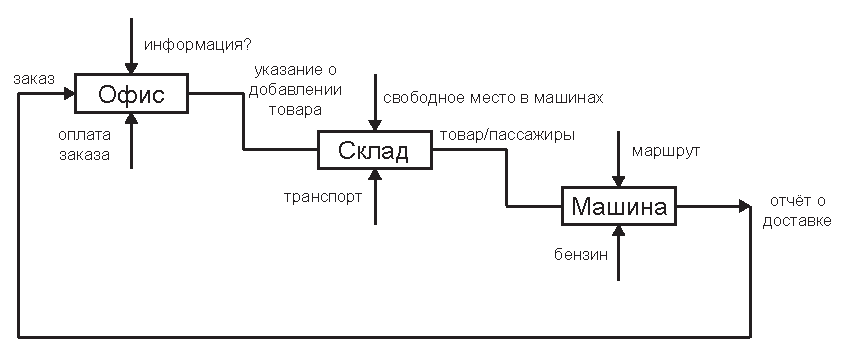
\includegraphics[width=.7\textwidth]{as_is_2}
    \end{figure}
\end{frame}

\begin{frame}
  \frametitle{Предложения}
  \begin{enumerate}
    \item автоматическое планирование маршрутов грузовых перевозок с учетом
      загруженности машины как в одну, так и в обратную сторону;
    \item создание списка рейсовых маршрутов как пассажирского, так и
      грузового транспорта;
    \item поддержка срочных частных заказов;
    \item отчетность об отбытии/прибытии в ключевые точки маршрута через БД.
  \end{enumerate}
\end{frame}

\begin{frame}
  \frametitle{TO BE}
    \begin{figure}
      \center
%      \includegraphics[width=.7\textwidth]{to_be}
    \end{figure}
\end{frame}

\begin{frame}
  \frametitle{Необходимые ресурсы}
\end{frame}

\begin{frame}
  \frametitle{Результат}
\end{frame}